\documentclass[handout]{beamer} % 16:9 aspect ratio for modern screens
% \documentclass[aspectratio=169]{beamer} % 16:9 aspect ratio for modern screens

% Theme settings
\usetheme[progressbar=foot]{metropolis} % Minimalist theme
\metroset{progressbar=frametitle} % Progress bar should only consider slides with titles?
\setbeamercolor{background canvas}{bg=white} % White background color

\makeatletter
    \setlength{\metropolis@progressinheadfoot@linewidth}{1.5pt}
\makeatother

\usefonttheme{professionalfonts} % Font theme

% Packages
\usepackage[T1]{fontenc}   % Font encoding
\usepackage[english]{babel} % English language
\usepackage[sfdefault]{FiraSans} % For FiraSans font
\usepackage[backend=biber, style=authoryear-comp
, sorting=nyt]{biblatex} % For bibliography
\usepackage{csquotes} % Recommended for biblatex with babel/polyglossia
\usepackage{textgreek} % Greek letters in text mode (from Citavi references)
\usepackage{tikz}          % For drawing graphics

\usepackage{graphicx}       % For including images
\usepackage{amsmath, amssymb} % For math symbols

\usepackage[labelformat=empty]{caption}

% Bibliography settings
\addbibresource{references.bib} % Path to the bibliography file

% Custom citation commands
\DeclareCiteCommand{\citeauthortitle}
  {\usebibmacro{prenote}}
  {\usebibmacro{citeindex}%
   \printnames{labelname}%
   \setunit{\space\textendash\space}
   \printfield{title}}
  {\multicitedelim}
  {\usebibmacro{postnote}}

\DeclareCiteCommand{\citeauthortitleurl}
  {\usebibmacro{prenote}}
  {\usebibmacro{citeindex}%
   \printnames{labelname}%
   \setunit{\space\textendash\space}
   \printfield{title}%
   \setunit{\addsemicolon\space}
   \printfield{url}}
  {\multicitedelim}
  {\usebibmacro{postnote}}

\DeclareCiteCommand{\parenciteauthortitle}
  {\usebibmacro{prenote}}
  {\bibopenparen\usebibmacro{citeindex}%
   \printnames{labelname}%
   \setunit{\space\textendash\space}% <- Here the separator ":" is added
   \printfield{title}\bibcloseparen}
  {\multicitedelim}
  {\usebibmacro{postnote}}

\makeatletter
\renewcommand\footnotesize{\tiny}
\makeatother

\newcommand{\figcite}[1]{\\[-3mm]{\tiny Source: \cite{#1}}}
\newcommand{\figciteweb}[1]{\\[-3mm]{\tiny from: \citeauthortitle{#1}}}
\newcommand{\figciteweburl}[1]{\\[-3mm]{\tiny from: \citeauthortitleurl{#1}}}

\mode<handout>{
    \AtBeginSection[]{} % In handout version, do not create section slides
}

% Title page settings
\title{TCBC: Temperature-Dependent SHG/THG Measurements}
\subtitle{Proof of Concept and Temperature Documentation}
\author{Florian Adamczyk}
\date{May 9, 2025}

\begin{document}

    % Black slide
    \begin{frame}<handout:0>[plain, noframenumbering]
        \begin{tikzpicture}[remember picture, overlay]
            \fill[black] (current page.south west) rectangle (current page.north east);
        \end{tikzpicture}
    \end{frame}

    % Appetizer Slide
    \begin{frame}<handout:0>[noframenumbering, plain]{Appetizer}
        \centering
        \includegraphics[width=\textwidth, height=0.9\textheight, keepaspectratio]{atom.jpg}
        \figciteweburl{Bonn.19.08.2021}
    \end{frame}

    % Title Slide
    \begin{frame}[noframenumbering, plain]
        \vspace*{-0.6cm}
        \titlepage
        \vspace*{-1.6cm}
    \end{frame}
    
    % Table of Contents
    \begin{frame}<handout:0>{Outline}
      \setcounter{page}{1}      
        \tableofcontents
    \end{frame}
    
    \section{Introduction}
    \begin{frame}{Motivation and Objectives}
      \begin{itemize}
        \item Investigation of TCBC using SHG/THG
        \item 1200nm and 1400nm laser light
        \item Proof of Concept for measurement setup and evaluation
        \item Temperature dependence of nonlinear optical properties
        
      \end{itemize}
    \end{frame}

    \section{Measurements and Results}

    % Image 1: SHG/THG at 1200nm
    \begin{frame}{SHG and THG Measurements at 1200nm (291K)}
      \begin{figure}
        \begin{minipage}{0.55\textwidth}
          \centering
          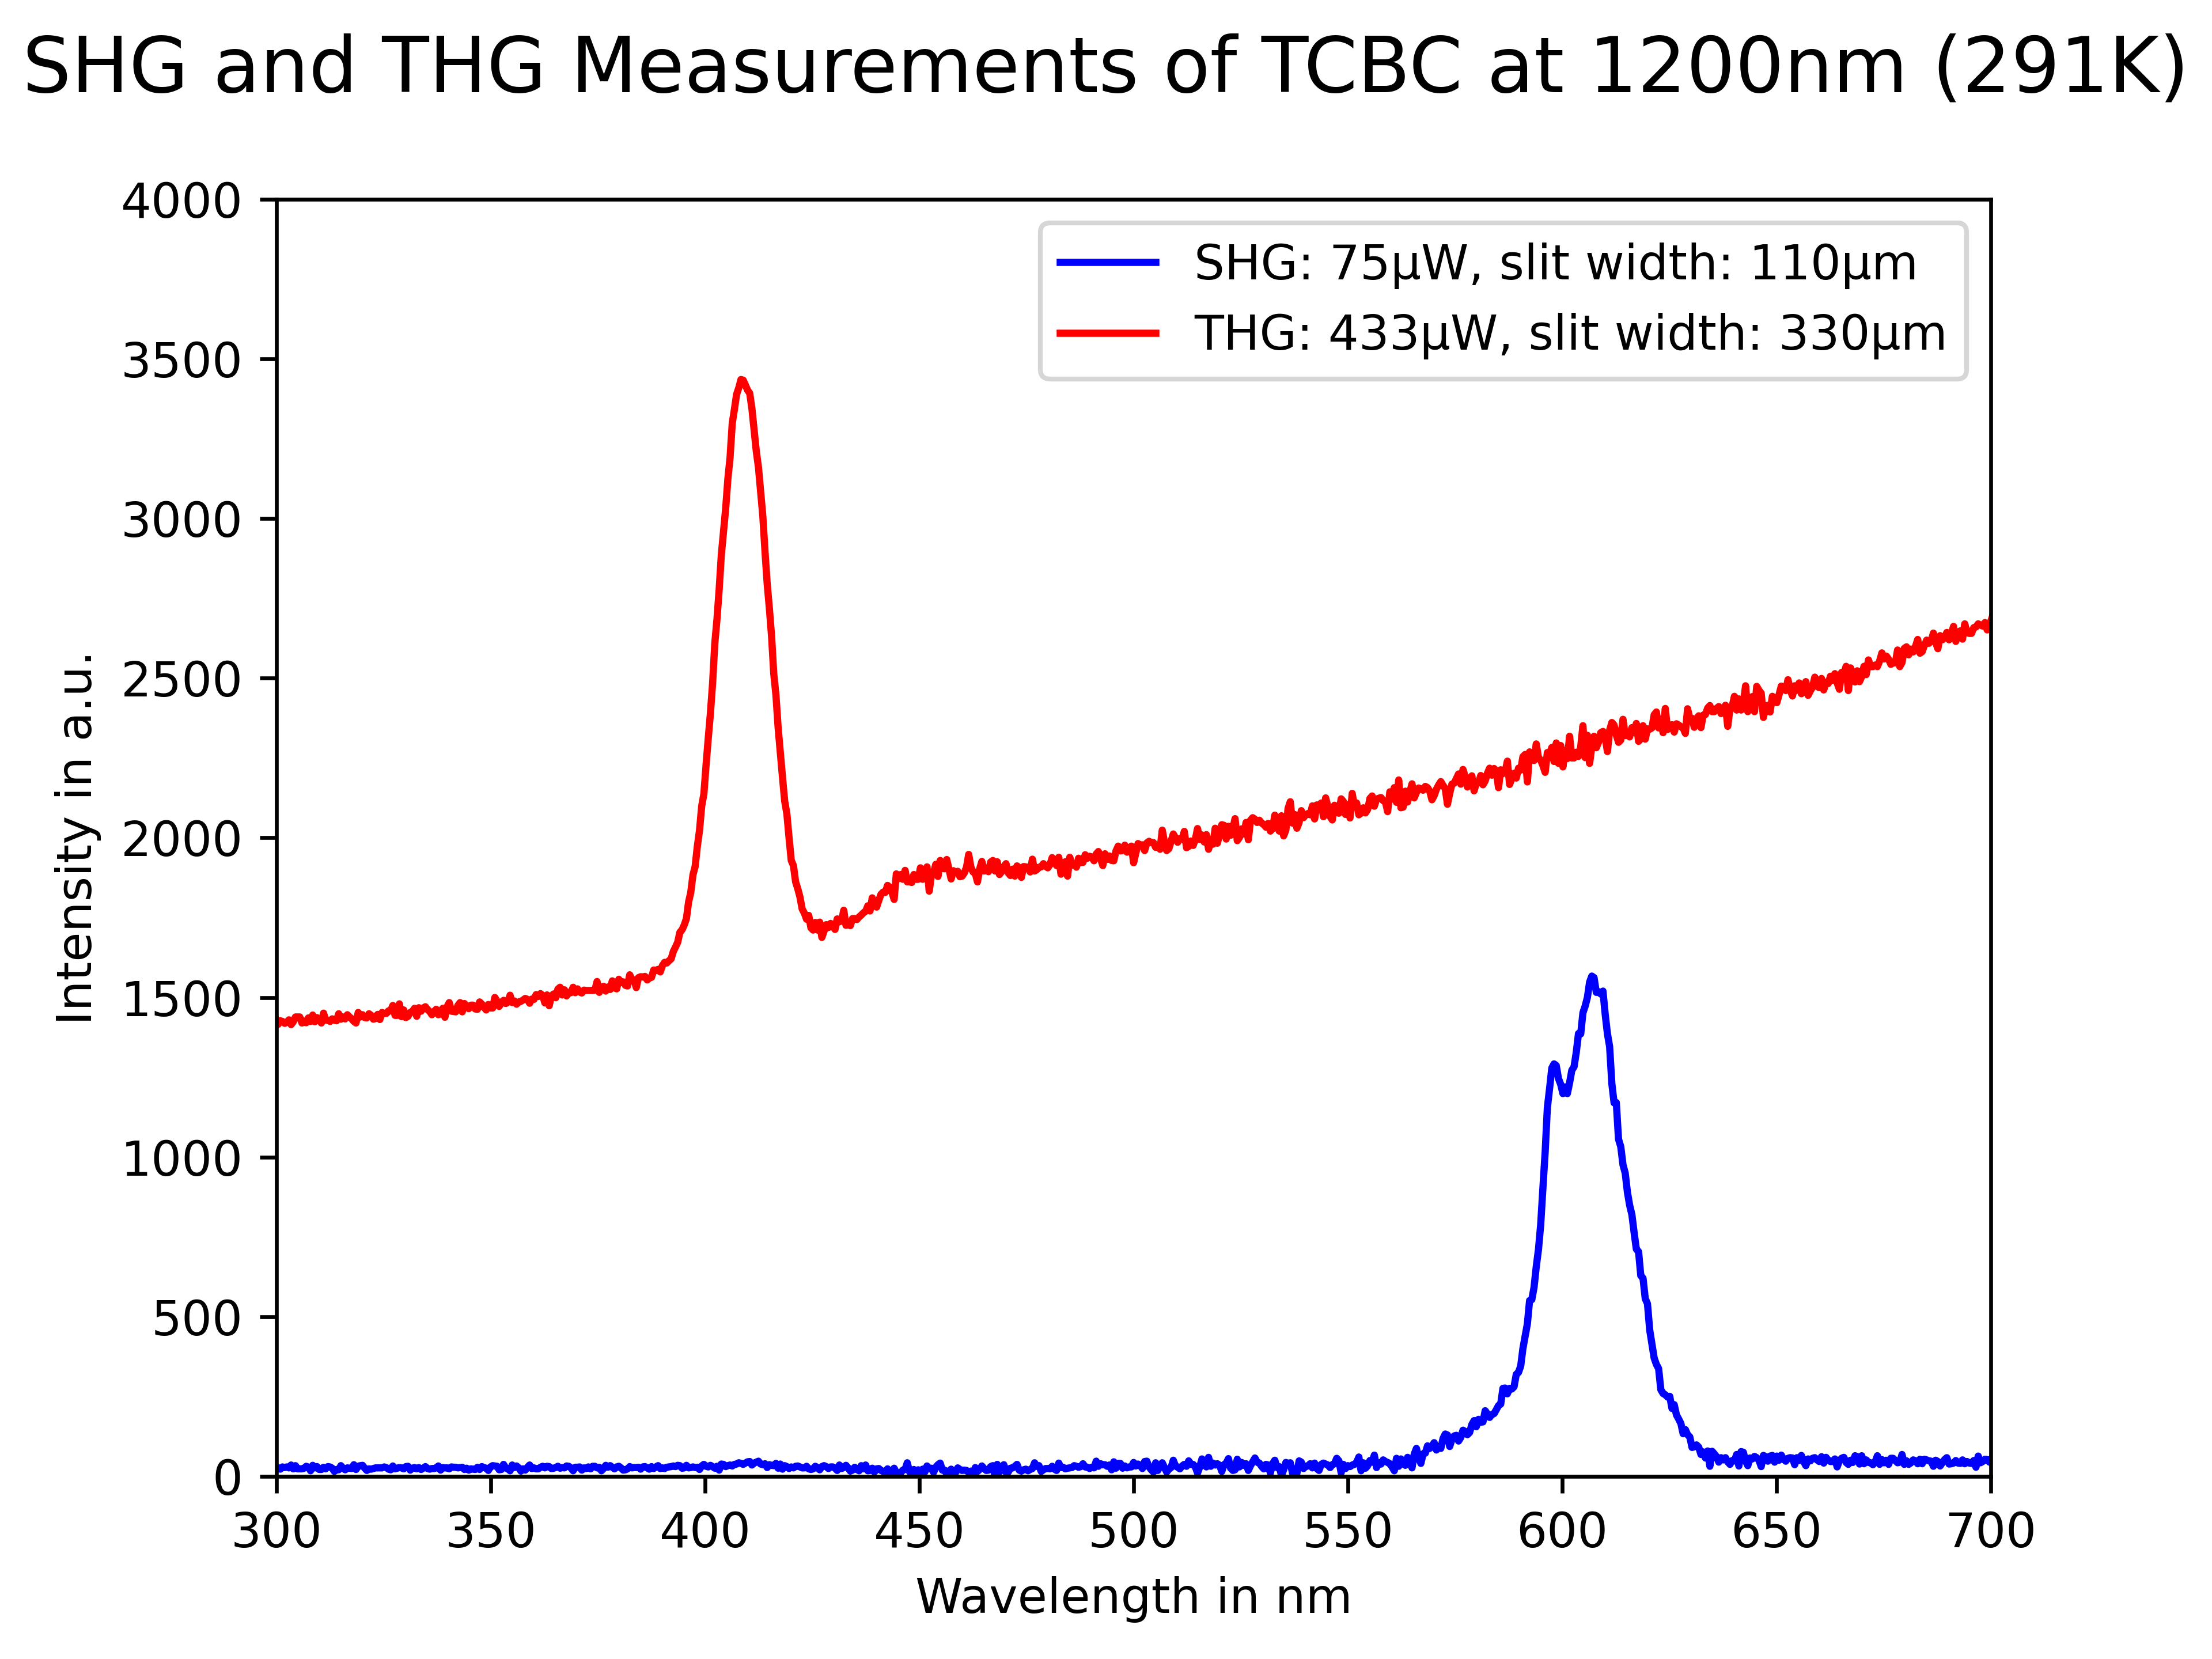
\includegraphics[width=\linewidth, keepaspectratio, height=0.85\textheight]{2025-05-08 TCBC 1200nm/TCBC_1200nm_combined_SHG_THG.png}
          \figciteweb{ownMeas1200}
        \end{minipage}
        \hfill
        \begin{minipage}{0.4\textwidth}
          \begin{itemize}
            \item Clear peaks at $\lambda_{SHG}$ and $\lambda_{THG}$
            \item For THG we needed a much higher Laser intensity and a larger slit width
            \item $\rightarrow$ the noise floor of the THG signal is much higher, and the crystal does white light generation due to the high intensity
          \end{itemize}
        \end{minipage}
      \end{figure}
    \end{frame}

    % Image 2: SHG at 1400nm, Temperature Series
    \begin{frame}{SHG Measurement at 1400nm: Temperature Dependence}
      \begin{figure}
        \centering
        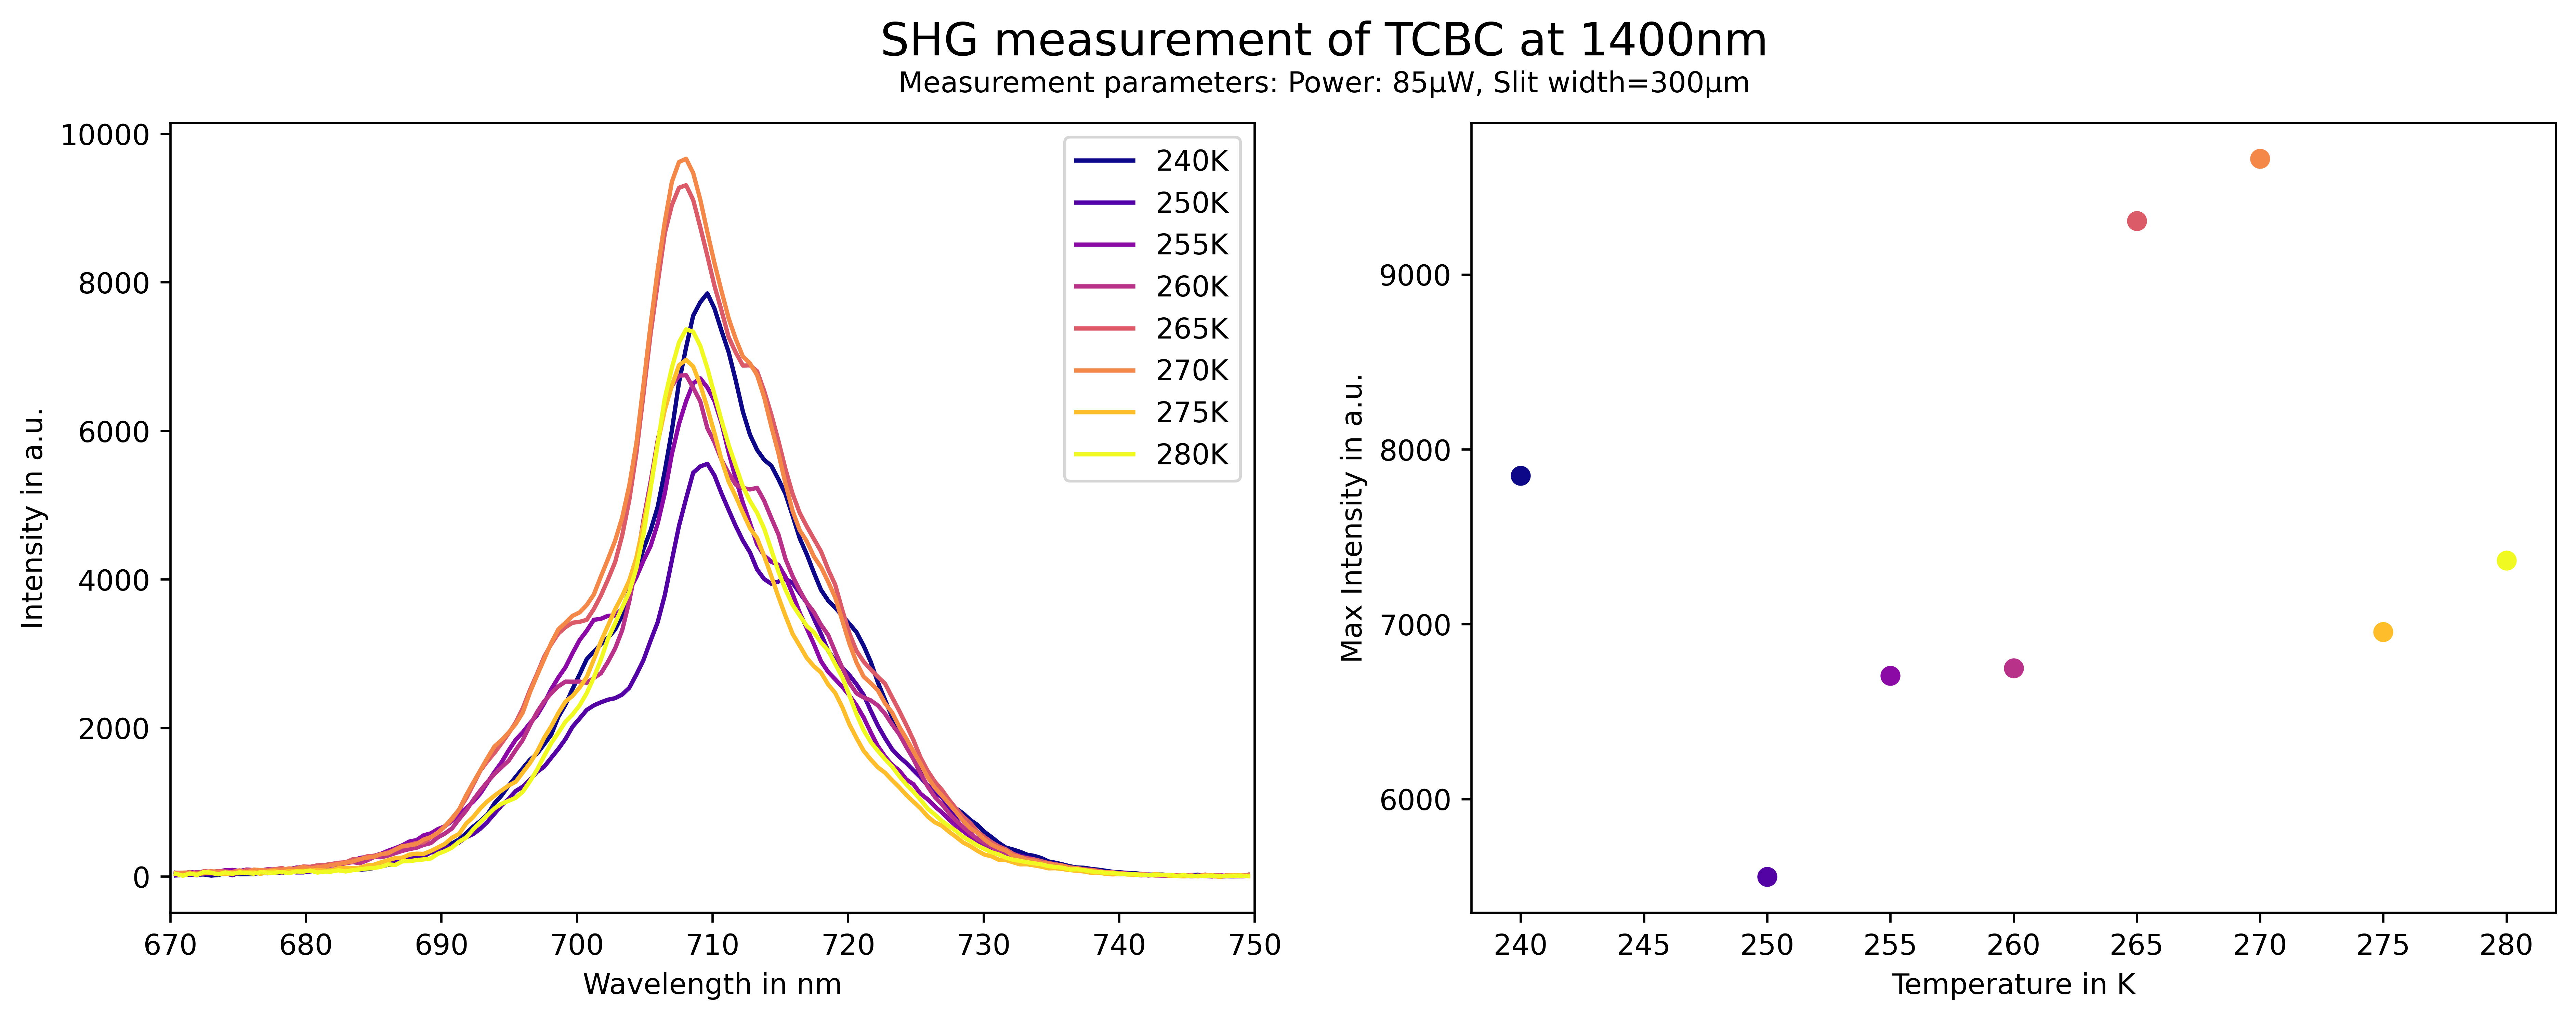
\includegraphics[width=0.85\textwidth, keepaspectratio, height=0.5\textheight]{2025-05-09 TCBC 1400nm ProofOfConcept/TCBC_SHG_ProofOfConcept.png}
        \figciteweb{SHGAndorSolis}
        \vspace{0.5em}
        \begin{minipage}{0.95\textwidth}
          \begin{itemize}
            % \item proof of concept for SHG measurement: Is a conclusive Measurement possible?
            \item Signal varies a lot because of shift of Probe due to thermal expansion
            \item Spot is too small to find the same crystal again resulting in a different signal each time
            \item Not suitable for temperature series
            \item \textbf{Conclusion:} We need to crush the crystals to a fine powder and measure the SHG/THG of the powder
          \end{itemize}
        \end{minipage}
      \end{figure}
    \end{frame}

    % Image 3: Temperature Profile during Measurement
    \begin{frame}{Temperature Profile during Measurement}
      \begin{figure}
        \begin{minipage}{0.55\textwidth}
          \centering
          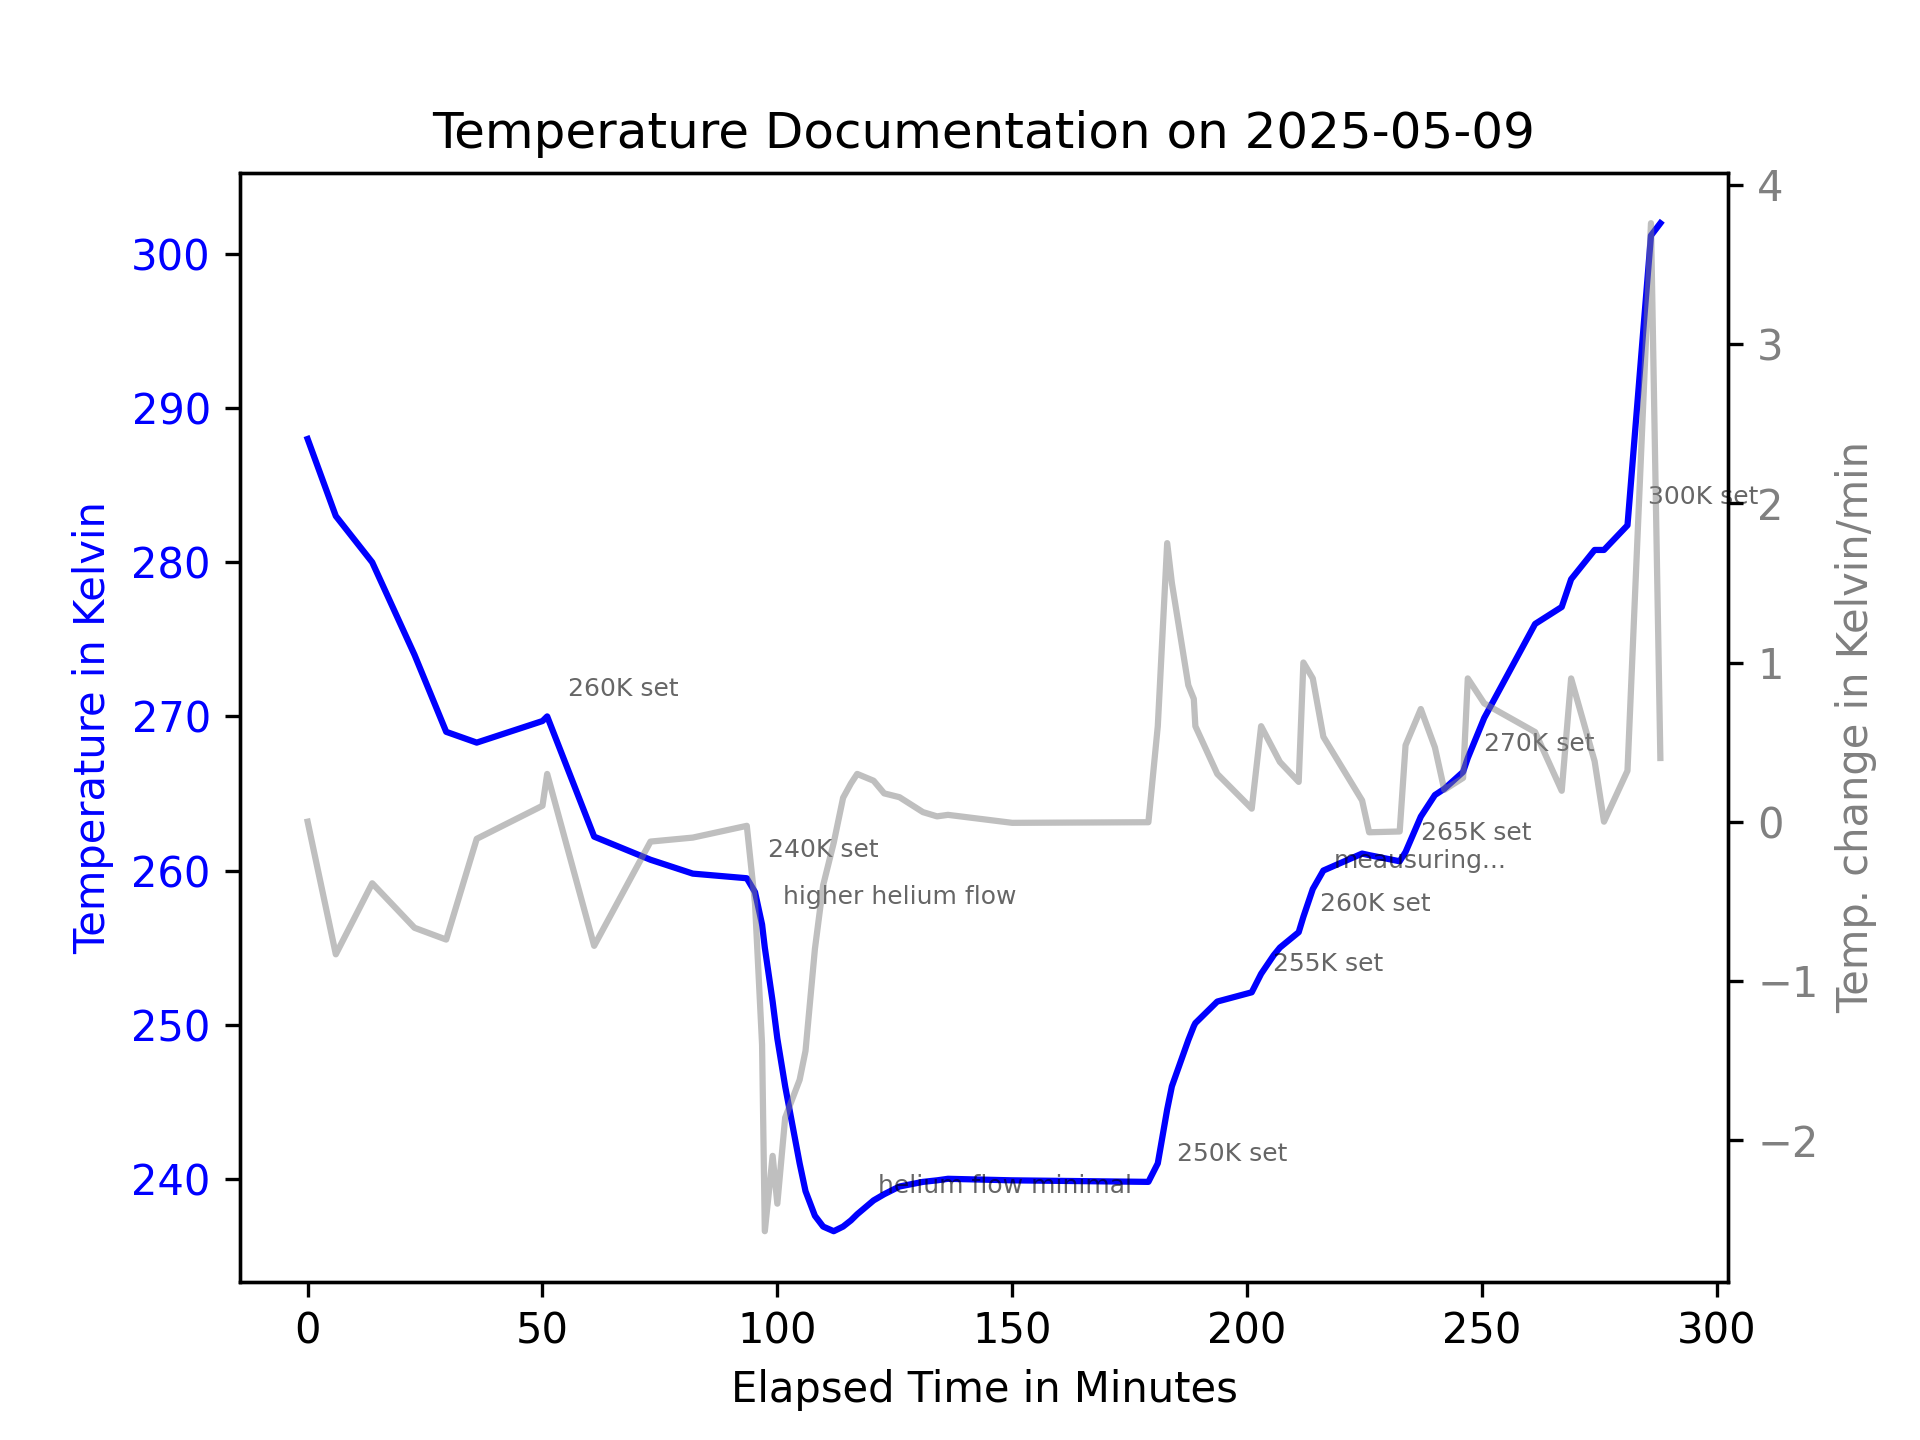
\includegraphics[width=\linewidth, keepaspectratio, height=0.85\textheight]{2025-05-09 TCBC 1400nm ProofOfConcept/Temperature Documentation/temperature_documentation.png}
          \figciteweb{TempMeas}
        \end{minipage}
        \hfill
        \begin{minipage}{0.4\textwidth}
          \begin{itemize}
            \item Documentation of temperature over time
            \item Annotations: Setpoints and special events
            \item Temperature change rate (gray, right axis)
            \item visible, that temperature change is always much slower than 10K/min.
          \end{itemize}
        \end{minipage}
      \end{figure}
    \end{frame}

    \section{Discussion}
    \begin{frame}{Interpretation of Results}
      \begin{itemize}
        \item It is very difficult to find the same spot on the crystal again
        \item Temperature change rate is very slow
        \item very few SHG spots which are very bright, mostly thg wich is only visible at very high intensities
        \item Crystals are too few in uncontrollable orientations
        \item maybe SHG is a surface effect and we need a larger surface area
        \item or maybe the orientation for SHG is very rare
      \end{itemize}
    \end{frame}

    \section{Conclusion}
    \begin{frame}{Conclusion and Outlook}
      \begin{itemize}
        \item Visible and strong SHG and THG signals at 1200nm

        \item Proof of Concept gave important insights
        \item We will crush the crystals to a fine powder and measure the SHG/THG of the powder
        \item that should give us a better signal because all orientations are present
        \item That will give a more reliable signal in variable temperature, eliminating the problem of finding the same spot on the crystal again
      \end{itemize}
    \end{frame}

    % Thank You Slide
    \begin{frame}<handout:0>{Thank you for your attention!}
      \begin{center}
        \Huge Questions?
      \end{center}
    \end{frame}

    % Black slide
    \begin{frame}<handout:0>[plain, noframenumbering]
      \begin{tikzpicture}[remember picture, overlay]
          \fill[black] (current page.south west) rectangle (current page.north east);
      \end{tikzpicture}
    \end{frame}

    % Appendix
    \begin{frame}<handout:0>[noframenumbering, plain, allowframebreaks]{Appendix}
      % Additional details, raw data, or supplementary plots can be inserted here.
      \begin{minipage}{0.4\textwidth}
        \textbf{Additional Notes}
        \begin{itemize}
          \item Details of the measurement setup
          \item Raw data
          \item References
        \end{itemize}
      \end{minipage}
      \hfill
      \begin{minipage}{0.58\textwidth}
        % Space for additional content
      \end{minipage}
    \end{frame}

    % Bibliography    
    \begin{frame}[allowframebreaks, noframenumbering, plain]{Literaturverzeichnis}
   \printbibliography%[nottype=unpublished]
    \end{frame}

\end{document}
